\documentclass[11pt,a4paper]{article}
\usepackage{color}
\usepackage{amsmath, amsthm, amssymb, amsfonts, verbatim}
\usepackage{graphicx}

\title{Assessing glymphatic transport velocities by adjoint methods}

\renewcommand{\comment}[1]{\textcolor{red}{#1}}

\author{Lars Magnus Valnes, Sebastian K. Mitusch, Geir A. Ringstad, Per Kristian Eide, Simon W. Funke, Kent-Andre Mardal }


\begin{document}
\maketitle

\begin{abstract}
\end{abstract}
\section{Introduction}

The discovery of the paravascular pathway in 2011~\cite{iliff2012paravascular} propose a novel component
crucial to the metabolism of the brain which may potientially provide an explanation for the accumulation of
waste such as amyloid beta in elderly, ultimately leading to diseases such as Alzheimer and Parkinson. 
In the rest of our body, the lymphatic system plays an important role
in the clearance of metabolic waste, but there are no lymphs within the brain. This fact is puzzling in particular because
the brain requires around 10 times more energy per volume than the result of the body. The paravascular 
pathway is proposed important to waste clearance and has therefore been named the \emph{glymphatic system}.      

The pioneering works of Sykov{\'a} and Nicholson~\cite{sykova2008diffusion} demonstrated
that diffusion was a governing transport mechanism in the brain. However, 
the clearance of CSF-tracers during sleep~\cite{xie2013sleep} in mice demonstrated transportation
much faster what could be explained by diffusion and it was proposed that arterial pulsation powered
accelrated perivascular flow combined convective interstitial flow. Several modelling attempts
have put the theory to the test~\cite{asgari2016glymphatic, smith2017glymphatic, holter2017interstitial}, 
but so far computational modeling have failed to adequately described the mechanism.   

Transportation by diffusion is in the order of XXX\comment{Lars: hente fra R. Thorne / Nicholson}. 
However, in \cite{xie2013sleep} a 60% coverage of 3kDa Texas Red Dextran of a $200 \mu m$ cube was demostrated in approximately 
20 minutes. As such, the transportation is XXX faster than what diffusion would provide. Furthermore, 
in \cite{eidevalnes} it was demonstrated that X Da Gadovist was brainwide in 8 hours after injection in the lumbar region.      

Paragraph about timescales etc. 

The purpose of this paper is to attempt to assess transportation speed in terms of an apparent diffusion coefficient 
by using adjoint methods provided by \cite{} for optimizing the coefficient with respect to data. As
such a coefficient larger than commonly reported values of diffusion would suggest that at the
timescale of minutes to hours there is indeed a glymphatic transportation which may potentially 
be responsible for metabolic waste.     

An outline of the paper is as follows. In Section 2 we descibe the medical images and their modality,  
and the mathematical methodology used for determining the apparent diffusion coefficients.  


\section{Methods}


\begin{itemize}
\item describe the imaging, shortly with ref to JCI  
\item describe the abstract mathematical problem to be solved, ie. PDE constrained opt problem where we 
address coefficients and bc  
\item the details: finite element, reduced problem, BFGS,  
\end{itemize}

\begin{figure}
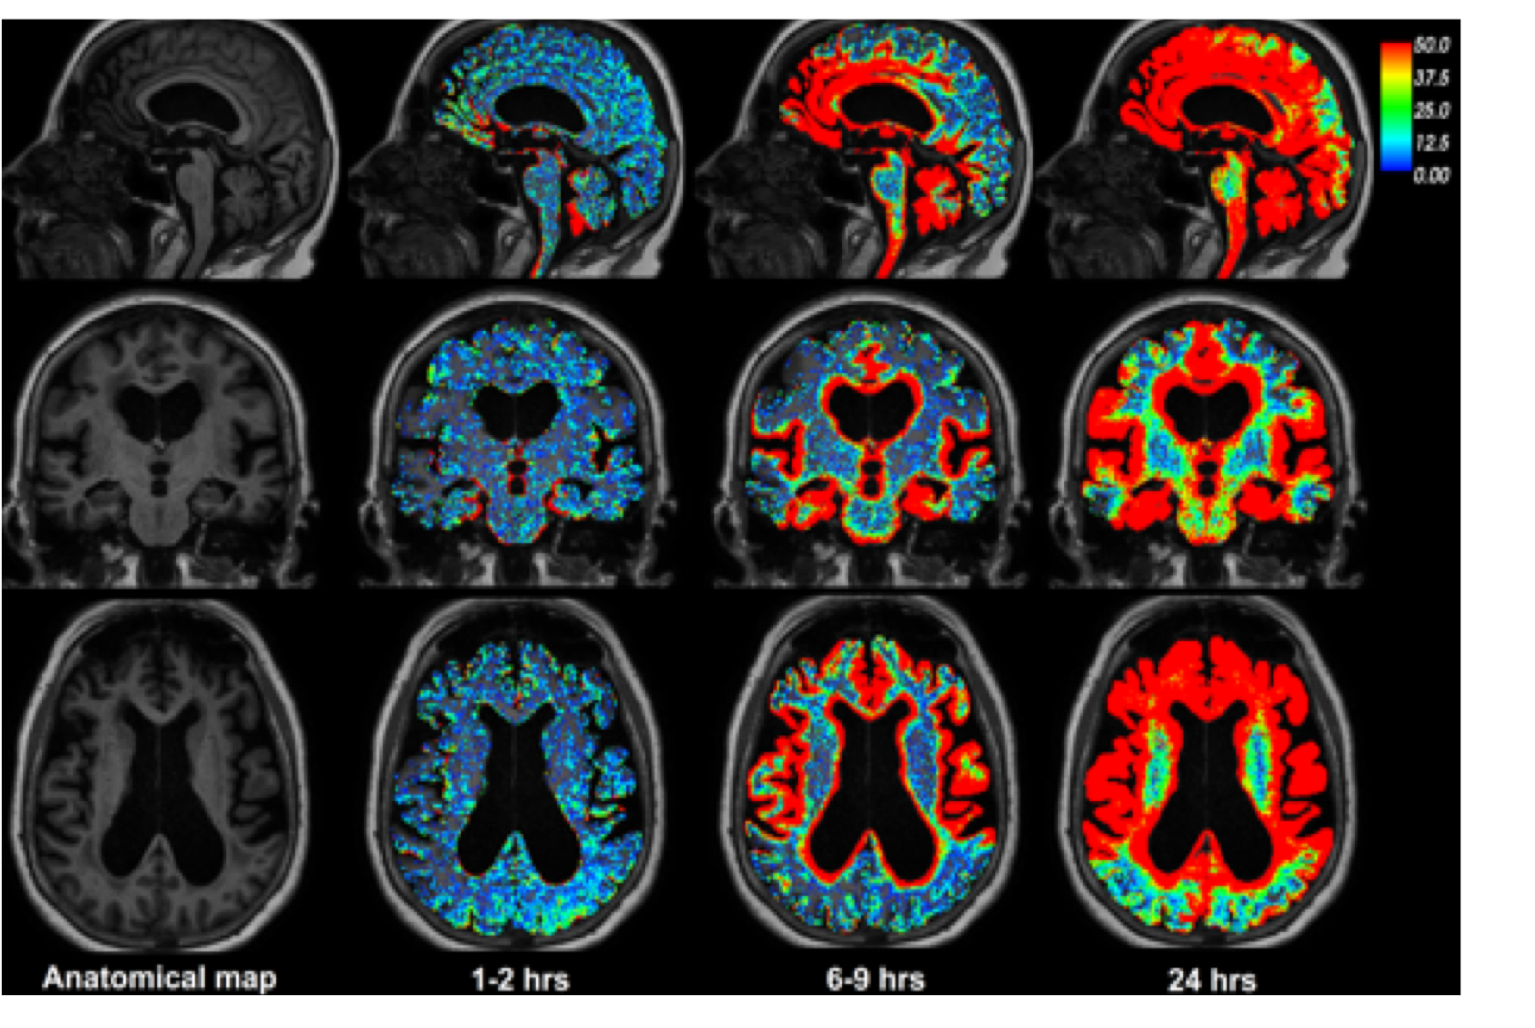
\includegraphics[width=0.95\textwidth]{GMRI.png} 
\label{fig1} 
\caption{\comment{lars, we will need some new images since I believe this is stolen from JCI}}
\end{figure}

\comment{Lars: bilde av konkret mesh }

\section{Results}
\begin{itemize}
\item 2D experiments as have already been done (with and without noise/ with and without observations everywhere in time) 
\item 2D experiments should highlight the impact of the regularization parameter wrt number of iterations and diffusion 
coeff 
\item 3D experiments based on data generated  
\item 3D experiments based on real data (\comment{lars: we need to try testing this}) 
\end{itemize}



\section{Discussion}

\bibliographystyle{amsplain}
\bibliography{references}


\end{document}


